\documentclass{article}
\usepackage{hyperref}
\usepackage{amsmath}
\usepackage{graphicx}
\begin{document}
\section*{Problem 2: GANs}
\subsection*{a. Architecture and Hyperparamters}
\
We used a DCGAN implementation from \href{https://pytorch.org/tutorials/beginner/dcgan_faces_tutorial.html}{PyTorch}.
They used the celeba dataset to train their DCGAN
and it was trained with these following hyperparameters:
\begin{center}
\begin{tabular}{|c|c|}
\hline
& Params for DCGAN Paper \\ \hline
Resolution & 64x64x3 \\ \hline
Latent Space Dim & 100 \\ \hline
Epochs & 5 \\ \hline
Learning Rate & 0.0002 \\ \hline
Beta1 (Adam) & 0.5 \\ \hline
Batch Size & 128 \\ \hline
\end{tabular}
\end{center}

The \href{https://arxiv.org/pdf/1511.06434.pdf}{paper for DCGAN} suggested the
hyperparameters of learning rate = 0.0002 and $beta_1=0.5$ so
the only hyperparameter that was changed from the source code was the number of epochs.
This depended on how many datapoints (images) were in the dataset. The celeba dataset
has about 200k images so 5 epochs were sufficient for them. Our dataset also had
200k images but with augmentation it doubled to 400k.
\subsubsection*{Issue 1 - Epochs was too low}
We thought that 3 epochs would be enough from the ratio of images to epochs. However, it 
was not enough to train the model as seen in the follow image:
\begin{center}
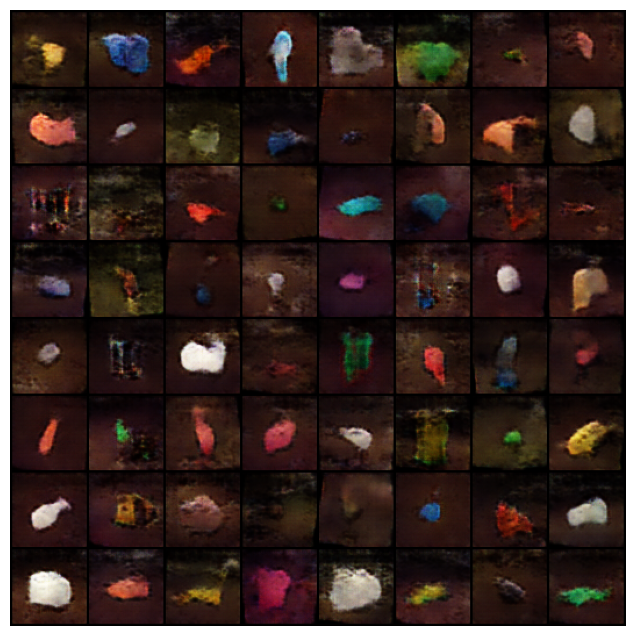
\includegraphics[scale=0.5]{./imgs/3epochs.png}
\end{center}
We assume that this is due to the variation between the legos is higher than the faces in celeba.

\subsubsection*{Issue 2 - Augmentation}
Realized that the diffusion model has its own Dataloader inside the pip package and thus we were
not able to apply the augmentations directly to the tensors when they were loaded in. Thus we decided
to not to use the augmentations due to not enough time to rewrite the entire package in the code.

\noindent Due to the two issues above, we have 200k images and decided to raise the number 
of epochs to 40 and thus our hyperparameters are:
\begin{center}
\begin{tabular}{|c|c|}
\hline
& Params for our DCGAN \\ \hline
Resolution & 64x64x3 \\ \hline
Latent Space Dim & 100 \\ \hline
Epochs & 40 \\ \hline
Learning Rate & 0.0002 \\ \hline
Beta1 (Adam) & 0.5 \\ \hline
Batch Size & 128 \\ \hline
\end{tabular}
\end{center}


\subsubsection*{Issue 3 - Resolution:}
I tried changing the dimensions of the data to a higher resolution but I couldn't resolve some error that popped up relating
to the dimensions of some vector and I wasn't able to fix it. So I decided to
keep the resolution at 64x64.

\subsubsection*{Issue 4 - Seeding:}
Heres the order of operations:
$$
\text{Seeding}
\rightarrow
\text{Training dataset augmentation and creation}
\rightarrow
\text{Fixed noise}
\rightarrow \dots
$$

\noindent This fixed noise was used to keep track of how the legos turned
out over time and since the dataset batching and augmentation happened before
the fixed noise, when trying to load the trained model, the fixed noise would look
different without the training dataset. The easy fix would be to change the order
at which it happens:
$$
\text{Seeding}
\rightarrow
\text{Fixed noise}
\rightarrow
\text{Training dataset augmentation and creation}
\rightarrow \dots
$$

\subsection*{b. Example Images}
TODO

We also decided to train a DCGAN on the VAE dataset:
TODO


\subsection*{c1. Interpolation}
Here is an interpolation between 4 different latent vectors:
\begin{center}
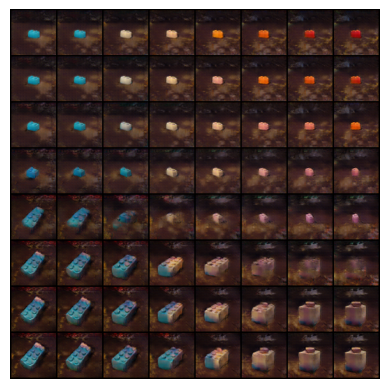
\includegraphics[scale=1]{./imgs/seed_69,0,23,42,62_interpolation}
\end{center}

\newpage
\subsubsection*{Issue 5 - Lego Inconsistency:}
Interpolating between these 4 legos:
\begin{center}
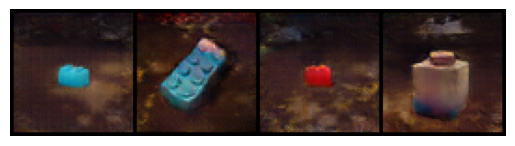
\includegraphics[scale=0.75]{./imgs/seed_69,0,23,42,62_legos}
\end{center}

\noindent The interpolation gave us legos that weren't the same as the input ones
(see the bottom right is green tipped instead of pink tipped):
\begin{center}
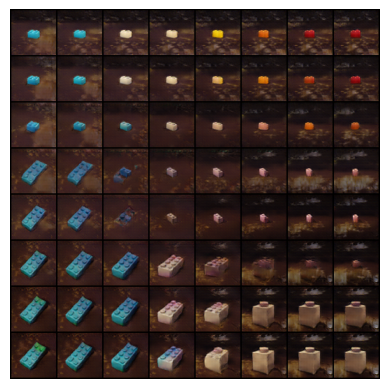
\includegraphics[scale=1]{./imgs/seed_69,0,23,42,62_wrong}
\end{center}

The network takes a $B$ (batch) sized of vector of latents and
converts it to batch of images
$$
(B \times d_z \times 1 \times 1)
\rightarrow_{G}
(B \times 3 \times 64 \times 64)
$$
The fix was to individually send each image through the network and combine the images
afterwards: 
$$
(1 \times d_z \times 1 \times 1)
\rightarrow_{G}
(1 \times 3 \times 64 \times 64)
$$

\subsection*{c2. Interpolation Video}
Generating many different latent vectors and interpolating between them in a video. See Box or Github for the mp4 file.
TODO LINK
\begin{center}
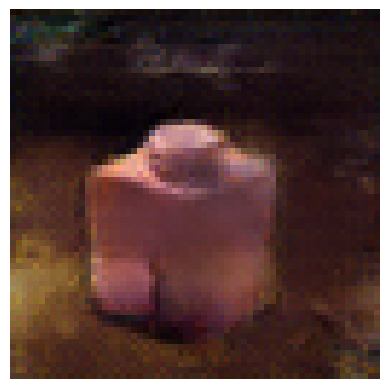
\includegraphics[scale=0.25]{./imgs/f1}
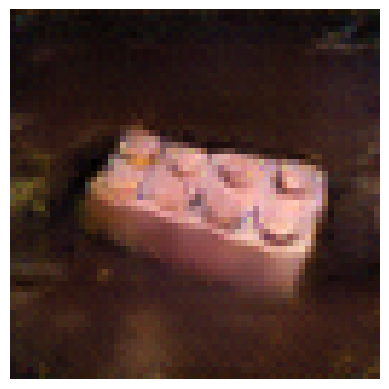
\includegraphics[scale=0.25]{./imgs/f2}
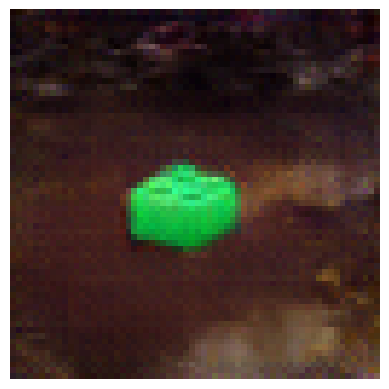
\includegraphics[scale=0.25]{./imgs/f3}
\end{center}

\subsection*{c3. Adding Constants to Latents}
TODO

\newpage
\section*{Problem 3: Diffusion Models}
\subsection*{a. Architecture and Hyperparamters}
We used a \href{https://arxiv.org/pdf/2006.11239.pdf}{Denoising Diffusion Probabilistic Model (DDPM)}. The original hyperparameters for
the \href{https://github.com/lucidrains/denoising-diffusion-pytorch}{DDPM repo} that we used were:
\begin{center}
\begin{tabular}{|c|c|}
\hline
& Params for repo DDPM \\ \hline
Resolution & 128x128x3 \\ \hline
Time Steps & 1000 \\ \hline
Training Steps & 700k \\ \hline
Learning Rate & 8e-5 \\ \hline
Ema Decay & 0.995 \\ \hline
Gradient Accumulate Every & 2 \\ \hline
\end{tabular}
\end{center}

\noindent We decided to keep the resolution the same as the GAN to
keep comparisons more fair. The only hyperparameter that we changed was
the training steps since 700k was going to take way too long
and 10k gave good results.

\begin{center}
\begin{tabular}{|c|c|}
\hline
& Params for repo DDPM \\ \hline
Resolution & 64x64x3 \\ \hline
Time Steps & 1000 \\ \hline
Training Steps & 20k \\ \hline
Learning Rate & 8e-5 \\ \hline
Ema Decay & 0.995 \\ \hline
Gradient Accumulate Every & 2 \\ \hline
\end{tabular}
\end{center}

\subsubsection*{Issue 6: Taking to long to train}
Started training the DDPM and it was 2k/700k steps and it had taken 5 hours.
The reason why cause it was doing FID Evaluations and they would take forever
since each image had 250 timesteps and there were 1500 evaluations.
I calculated that would it would take approx 60 days to train with evaluations. The fix was to
just turn off the evaluations by setting it to False.

\subsection*{b. Example Images}
TODO

\subsubsection*{Issue 7: VRAM Issues}
I was running out of VRAM when generating more than 5 images at a time. The fix was to
generate one image at a time, bring it to CPU/RAM and clear the cache in the GPU.

\subsection*{c1. Interpolation}
Here is an interpolation between two different latent spaces:
TODO
Compared to the GAN and VAE, the diffusion interpolation happens very suddenly.

\subsection*{c2. Interpolation Video}
As with the GAN we created a video of the interpolation between many different latent spaces on Box and Github.
TODO LINK and IMages

\end{document}